\section{Proof-of-concept (PoC) system}\label{sec:poc_system}
The proof-of-concept (PoC) system is a web-based application that allows users to search for products, view their price history, and compare prices across different websites.
It includes a user interface which provides the following features:
\begin{itemize}
    \item A search bar that allows users to enter a product name or keyword to search for products across different websites.
    \item A product list page that displays the search results, including product name, price, image, and stock status.
    \item A product detail page that displays the product's price history, including a graph of the price changes over time and a table of historical prices.
    \item A similar products section that displays a list of identical products from different websites, allowing users to compare prices and make informed purchasing decisions.
    \item A metadata section that displays additional information about the product page's lifecycle, which includes the dates and times of the last crawl, mininimization, classification and information extraction.
    \item A side-by-side view of the original and minimized HTML content of the product page, allowing users to see the differences between the two versions.
\end{itemize}

The front-end of the application is build using Next.Js, a popular framework for building web applications, and is hosted using AWS Amplify, a cloud-based platform for building and deploying web applications.
The back-end (API) is built using Golang with the Mux router, a lightweight and efficient HTTP router for building RESTful APIs.
It is hosted using AWS Lambda, a serverless computing platform that allows for scalable and cost-effective deployment of APIs.
The API is fronted by an AWS API Gateway, which provides a secure and scalable entry point for the API, and also handles rate limiting to prevent abuse and ensure fair usage of the system.

The API provides the following endpoints:
\begin{itemize}
    \item \texttt{GET /products?url={url}} - Retrieves product information based on the provided URL.
    \item \texttt{GET /products/search?query={query}} - Searches for products based on the provided query.
    \item \texttt{GET /products/history?url={url}} - Retrieves the price history of a product based on the provided URL.
    \item \texttt{GET /products/similar?url={url}} - Retrieves a list of similar products based on the provided URL.
    \item \texttt{GET /products/metadata?url={url}} - Retrieves metadata information about the product page's lifecycle based on the provided URL.
    \item \texttt{GET /products/source-crawled-page?url={url}} - Retrieves the original crawled HTML content of the product page based on the provided URL.
    \item \texttt{GET /products/source-minimized-page?url={url}} - Retrieves the minimized HTML content of the product page based on the provided URL.
    \item \texttt{GET /products/random} - Retrieves a random product from the database.
    \item \texttt{POST /products/mark-matching?url1={url1}\&url2={url2}\&isMatching={match}} - Marks two products as matching based on the provided URLs and match status.
\end{itemize}

Figure~\ref{fig:poc_system} illustrates the architecture of the proof-of-concept (PoC) system, showing the interactions between the front-end, back-end, and various AWS services used for hosting and deployment.

\begin{figure}[H]
    \centering
    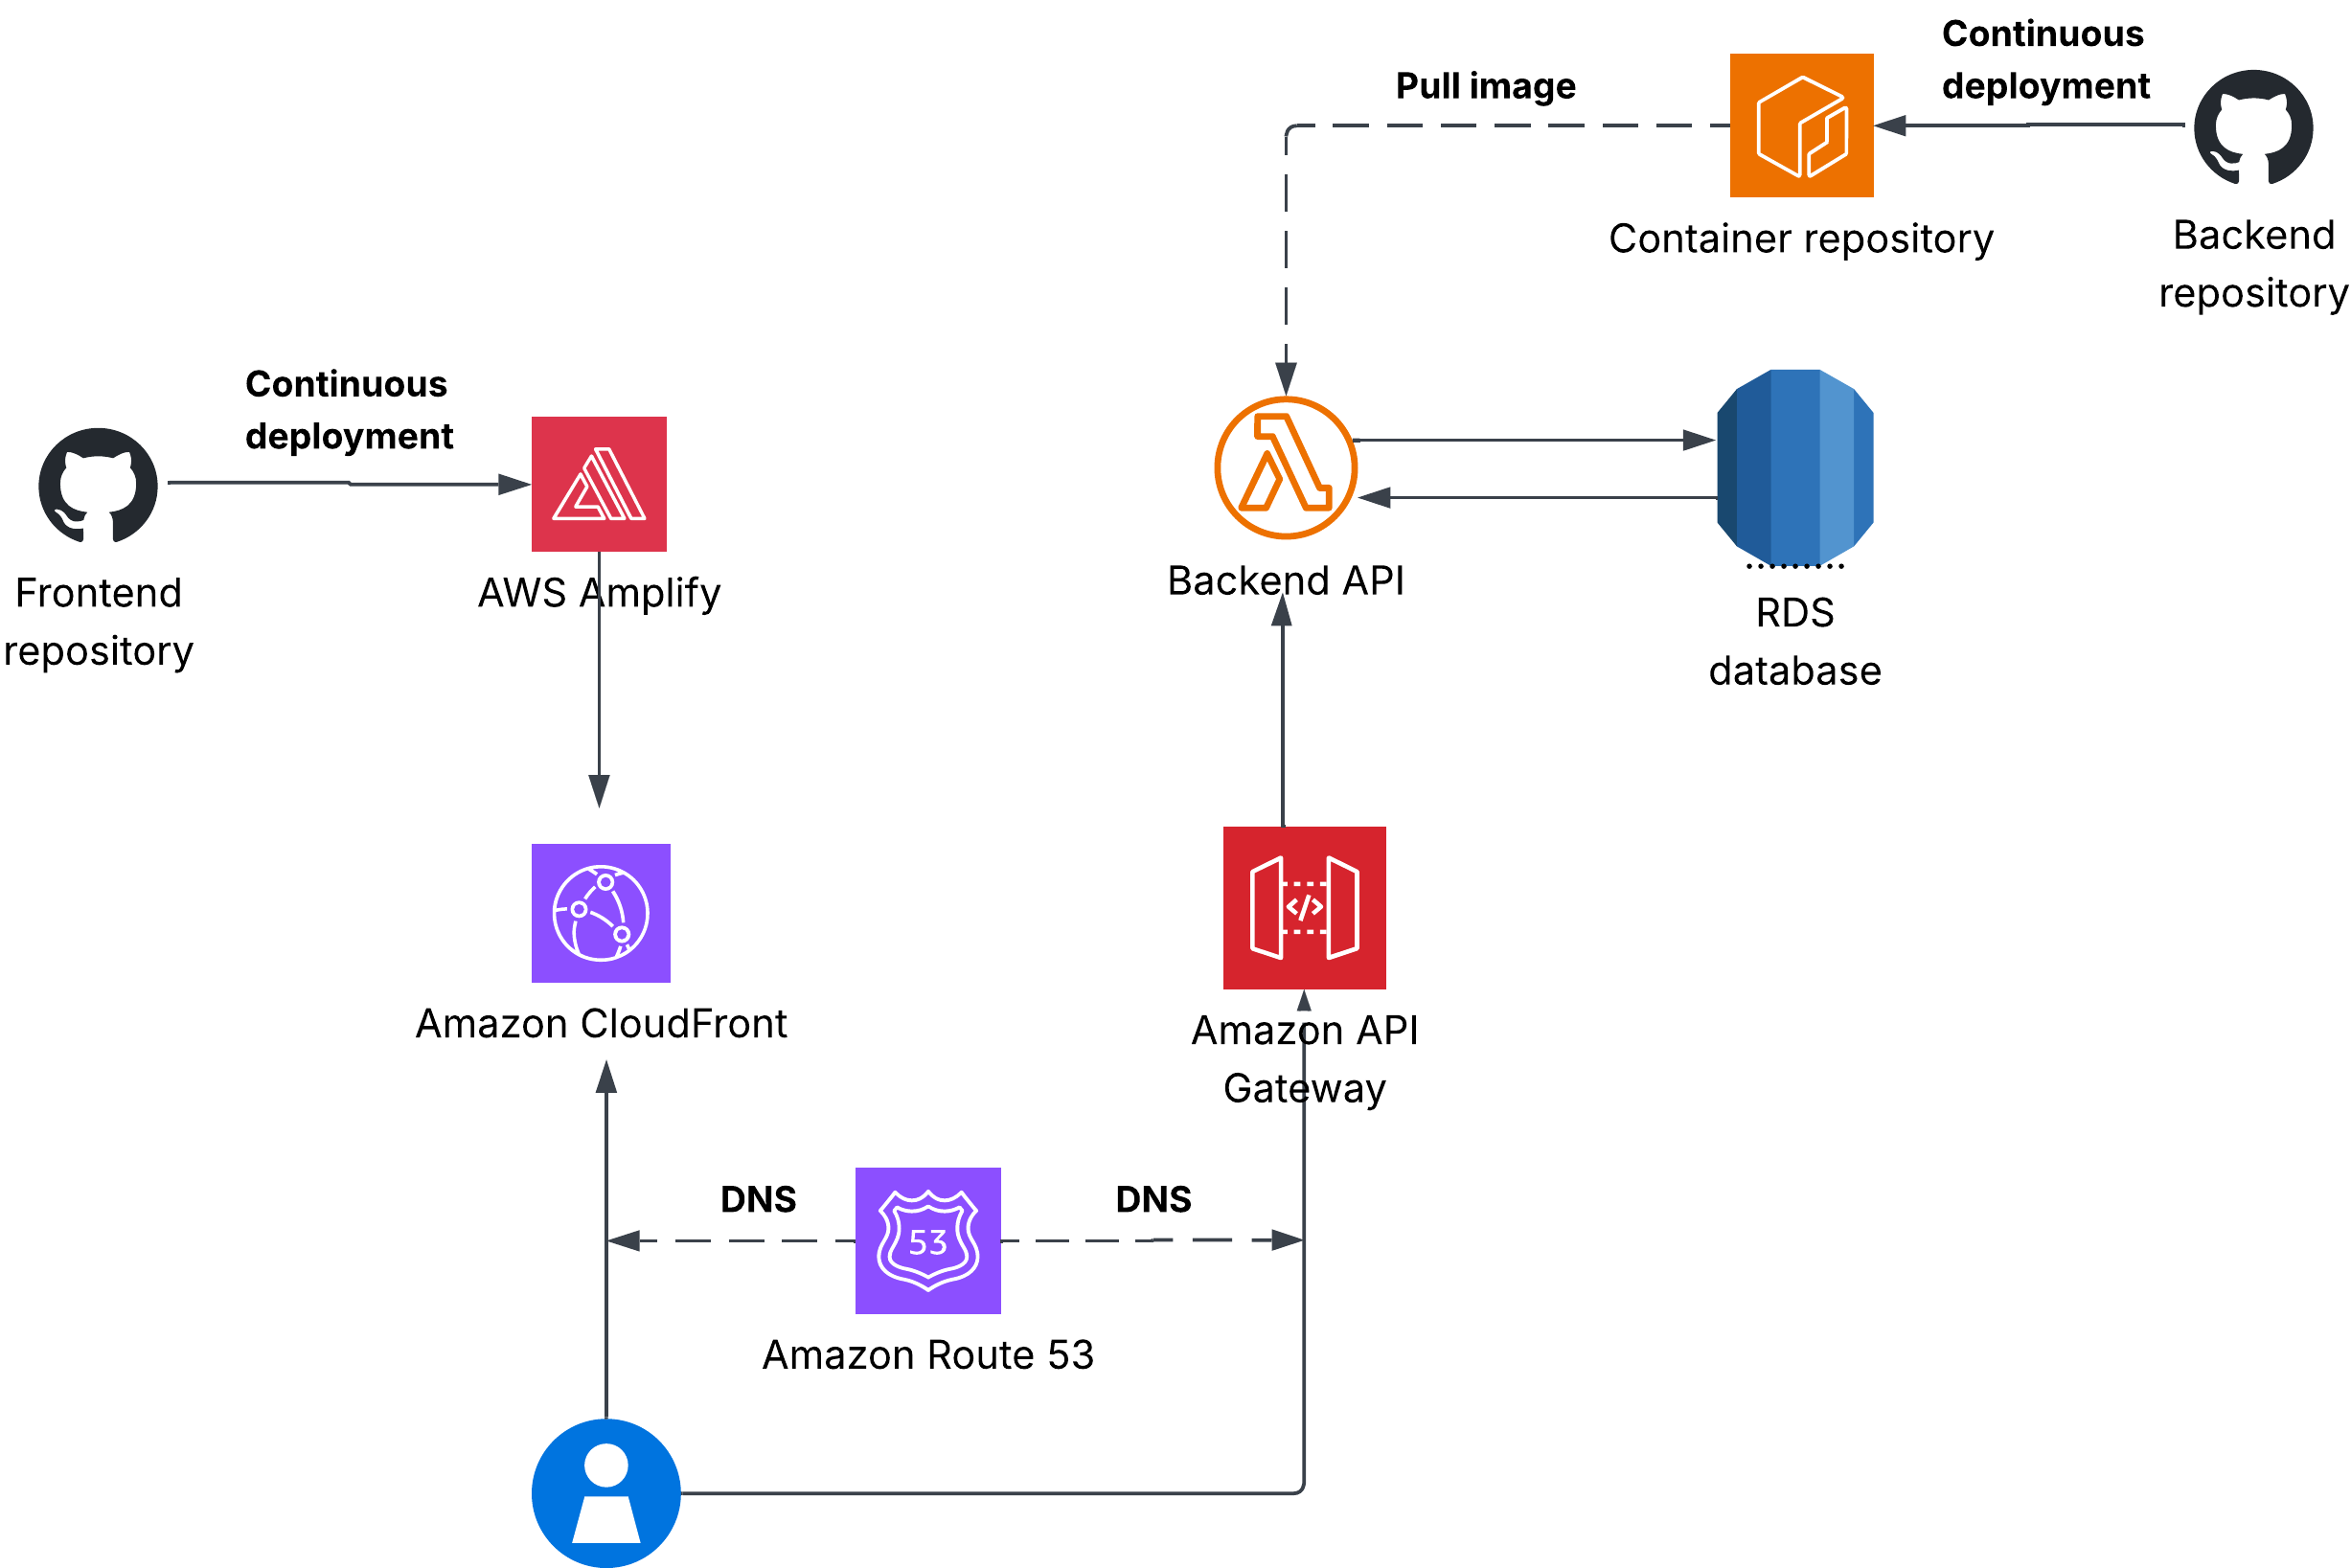
\includegraphics[width=0.8\textwidth]{images/poc_architecture}
    \caption{Proof-of-concept (PoC) system architecture}
    \label{fig:poc_system}
\end{figure}